In this section, we discuss the simulation performances of the algorithms briefed in Section \ref{sec-3} and \ref{sec-4}. The comparison studies are made using the queue deviation and sum rate convergence of the algorithms discussed so far using different system models. The distributed algorithms for the \ac{JSFRA} scheme and the equivalent \ac{MSE} representation are compared using the excess backlogged packets present after the current iteration instant.

Fig. \ref{fig-d-1} demonstrates the performance of the distributed algorithms in an \ac{OFDM} framework modeled with \me{N = 5} sub-channels with \me{N_B = 2} \acp{BS}, each equipped with \me{N_T = 4} transmit antennas. Each \ac{BS} serves \me{|\mc{U}_b| = 4, \forall b \in \{1,2\}} users in a coordinated manner so as to minimize the interference caused to the neighboring \ac{BS} users. Fig. \ref{fig-d-1.1} shows the total number of backlogged packets at the end of each iteration and Fig. \ref{fig-d-1.2} plots the total rate achieved by various algorithms at each iteration. As discussed earlier in the distributed section, the rate of convergence of any distributed algorithm depends on the proper choice of a step size. In particular, the primal decomposition method is more susceptible to the choice of the step size compared to the \ac{ADMM} approach. Since the primal decomposition iterates at each instant by fixing the interference thresholds, it may lead to infeasible solutions if the initial interference values are not feasible and also with the updated interference value as in \eqref{primal-sg-update}.

Fig. \ref{fig-d-1} also compares the performance of the iterative algorithm for \ac{JSFRA} scheme via \ac{MSE} reformulation using the \ac{KKT} conditions discussed in Section \ref{sec-4.3}. The performance is inferior compared to the other algorithms due to the violation in the assumptions made in the algorithm design \textit{i.e}, \me{Q_k \gg t_k}. Since in this case, we are comparing the \me{q = 1} case, the queue condition \me{Q_k \gg t_k} needs to be satisfied in order to remove the absolute operator from the expression in \eqref{eqn-9.1a} to form \eqref{kkt-mse-1.1}. The total number of backlogged packets after the each iteration reduces monotonically in all cases and converges to the points closer to the centralized solution \me{\chi = 33} bits. As seen in Fig. \ref{fig-d-1}, the \ac{ADMM} approach provides better convergence compared to the primal approach in the initial phase due to the quadratic penalty term included in the objective, which gets pronounced initially due to the large deviation between the assumed and the actual interference across the coordinating \acp{BS}.
\begin{figure*}
\centering
\begin{subfigure}{0.49\textwidth}
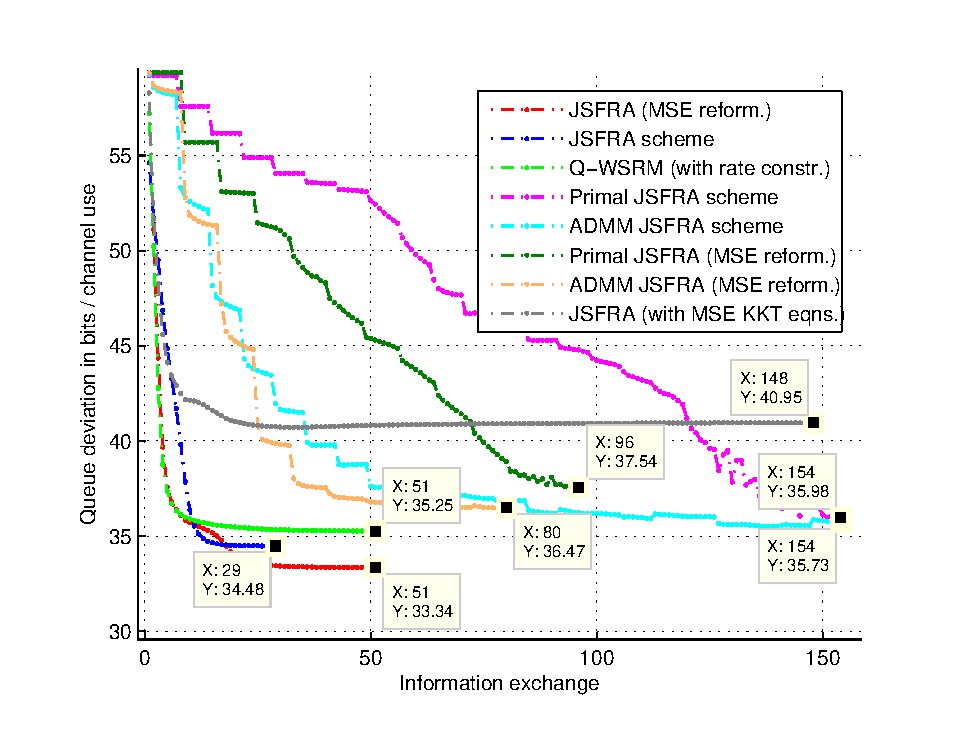
\includegraphics[width=\columnwidth]{NewFigures/distribute_queue-1}
\caption{Queue deviation}
\label{fig-d-1.1}
\end{subfigure}
\hfill
\begin{subfigure}{0.49\textwidth}
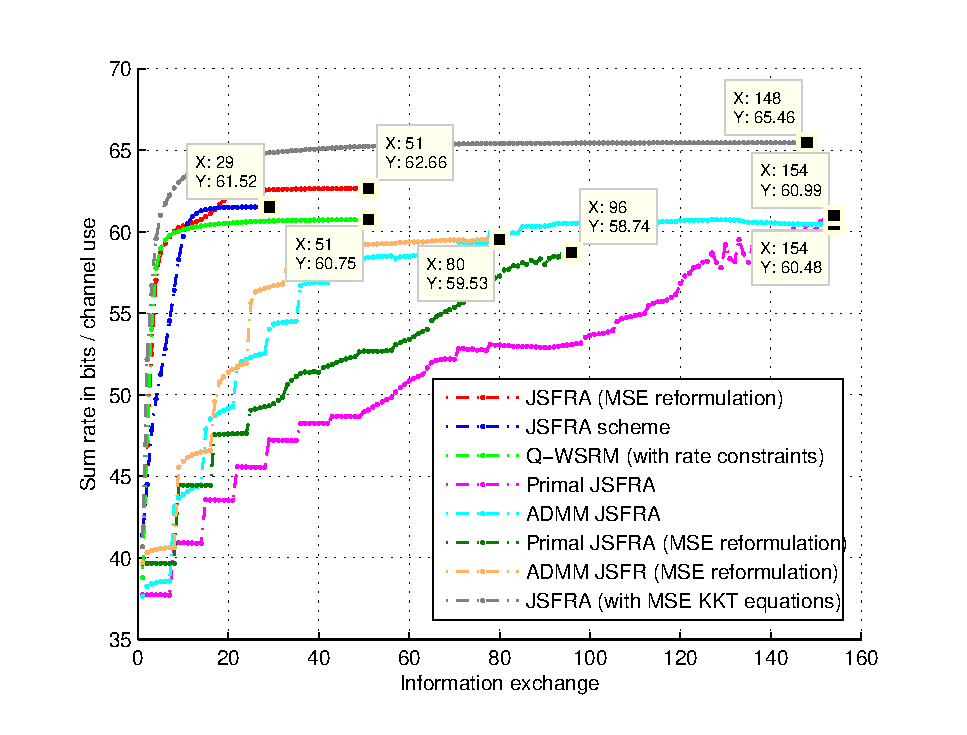
\includegraphics[width=\columnwidth]{NewFigures/distribute_sum_rate-1}
\caption{Sum rate performance}
\label{fig-d-1.2}
\end{subfigure}
\caption[short]{Convergence plot for \me{\lbrace N,N_B,K,N_R \rbrace = \lbrace 5,2,8,1 \rbrace} model}
\label{fig-d-1}
\end{figure*}

In Fig. \ref{fig-d-2}, the total backlogged packets and the sum throughput offered to minimize the number of queued packets for \me{K = 12} users across \me{N = 5} sub-channels are plotted for the analysis. The system considers \me{N_B = 3} \acp{BS}, each having \me{N_T = 4} transmit antennas serving \me{|\mc{U}_b| = 4} users mounted with \me{N_R = 2} antennas respectively. The users are assumed to be scattered over the cell boundary with the maximum interference power from any neighboring \ac{BS} follows \me{\mathbb{U}(0,-6)} dB independently. The sum rate and queue minimizing behavior follows similar pattern as in Fig. \ref{fig-d-1} for \me{N_B = 2} \acp{BS} scenario.

Fig. \ref{fig-d-2} demonstrates the convergence behavior of the different distributed algorithms discussed so far. It can be seen from Fig. \ref{fig-d-2}, that the distributed algorithms depend on the step size used in the subgradient update procedure. The primal decomposition algorithm, which distributes the precoder design by fixing the interference thresholds at each iteration, converges to the optimal resource allocations gradually as compared to the \ac{ADMM} based dual approach. The \ac{ADMM} scheme depends on the step size for the convergence, where the larger step size makes the algorithm to reach the optimal point quickly but takes more iterations to converge. The choice of \me{I_{\max}}, which denotes the maximum \ac{SCA} iterations, and the \me{J_{\max}}, which denotes the subgradient convergence limit, are fixed at \me{100} and \me{8} respectively. The information exchange is made at each instant and the performances are evaluated as if the actual transmission is happened with the precoders \me{\mvec{m}{l,k,n}^{(i)}} designed at the \me{\ith{i}} instant in a distributed manner. In this paper, we assume that the actual transmission will happen at the end of the precoder convergence or when the maximum number of iterations reached.

The performance of the joint \ac{Q-WSRM} scheme discussed in the Section \ref{sec-3.1} performs slightly worse than (\me{\approx \, 2} bits) the \ac{JSFRA} scheme in reducing the number of queued packets, even though the performance were similar in Table \ref{tbl-1}. As stated earlier, the joint \ac{Q-WSRM} scheme and the \ac{JSFRA} scheme with the exponent \me{q = 1} performs the same when the number of queued packets are identical for all the users. In this case, the joint \ac{Q-WSRM} becomes the sum rate maximization problem which is equivalent to the greedy \me{q=1} \ac{JSFRA} scheme. In the current scenario, since the number of queued packets are different for the users, the performance of the \ac{JSFRA} scheme is better due to its greedy resource allocation. It can be seen from Fig. \ref{fig-d-2}, that the \ac{KKT} based approach provides inferior result in the queue minimization perspective as compared with the sum rate plot. The performance degradation is due to the unconstrained rate increase for the users beyond their actual number of queued packets available to transmit. Since the objective uses the norm-\me{1} minimization, the \ac{KKT} solution is not optimal unless the queues are far greater than the transmission rate available for each user. The number of queued packets are initialized in a way to analyze the effect of the unconstrained behavior in the \ac{KKT} scheme.
\begin{figure*}
\centering
\begin{subfigure}{0.49\textwidth}
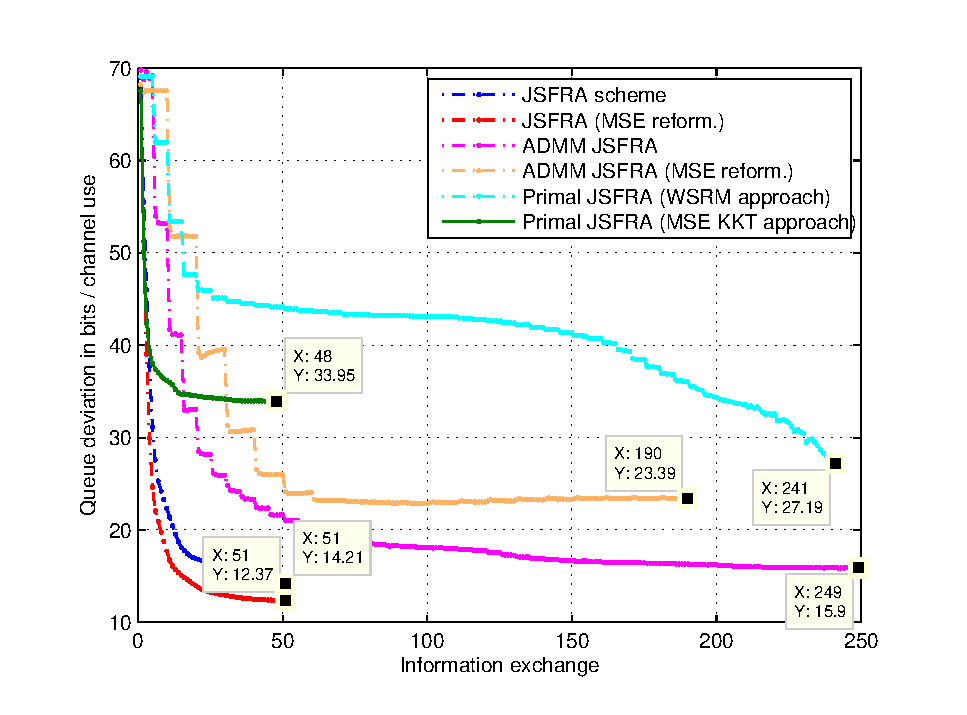
\includegraphics[width=\textwidth]{NewFigures/distributed_queue_plot_1}
\caption{Queue deviation}
\end{subfigure}
\hfill
\begin{subfigure}{0.49\textwidth}
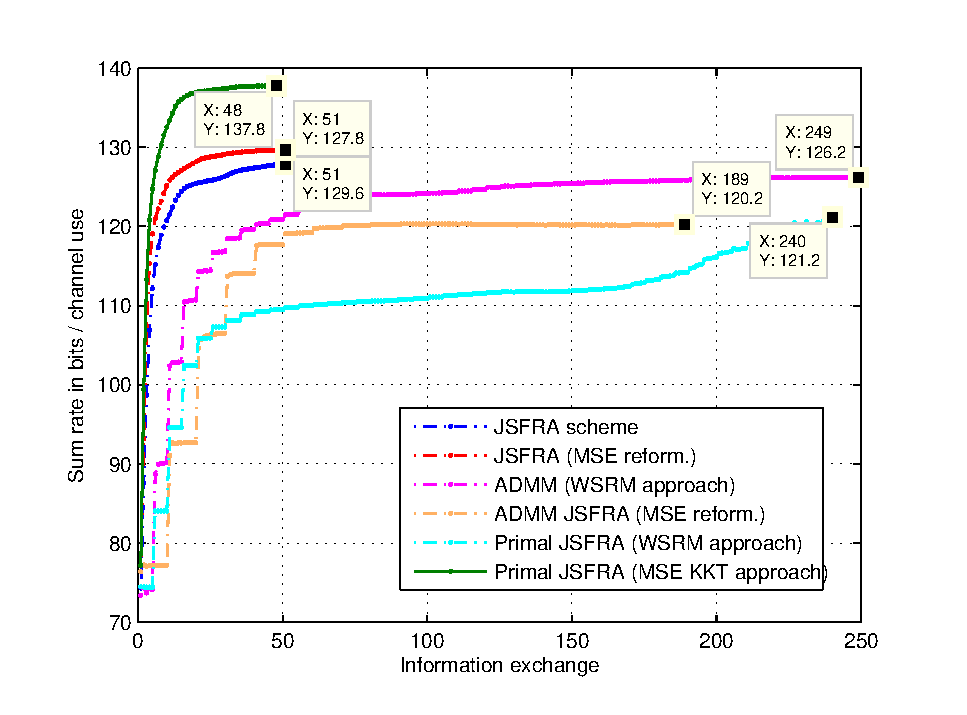
\includegraphics[width=\textwidth]{NewFigures/distributed_sum_rate_plot_1}
\caption{Sum rate performance}
\end{subfigure}
\caption{Convergence plot for \me{\lbrace N,N_B,K,N_R \rbrace = \lbrace 5,3,12,2 \rbrace} model}
\label{fig-d-2}
\end{figure*}

The performance of the \ac{MSE}-\ac{KKT} scheme is shown in comparison with the other schemes discussed so far in Fig. \ref{fig-d-3}. It can be seen that the \ac{KKT} based approach performs similar to the optimization problem given in \eqref{eqn-9}, which is solved using the solver \cite{grant2008cvx}. In the two norm case, the objective is differentiable and hence can be differentiable for any number of queued packets as compared to the one norm case requiring larger queue sizes in order to drop the absolute function occurring in the norm function. The performance of the closed form solution using the \ac{KKT} solution achieves similar performance without allocating rates beyond the available queued packets. In order to bring out the performance difference, one norm objective plot is also provided in Fig. \ref{fig-d-3} providing better reduction in the number of queued packets in the current transmission slot.
Fig. \ref{fig-d-3}
\begin{figure*}
\centering
\begin{subfigure}{0.49\textwidth}
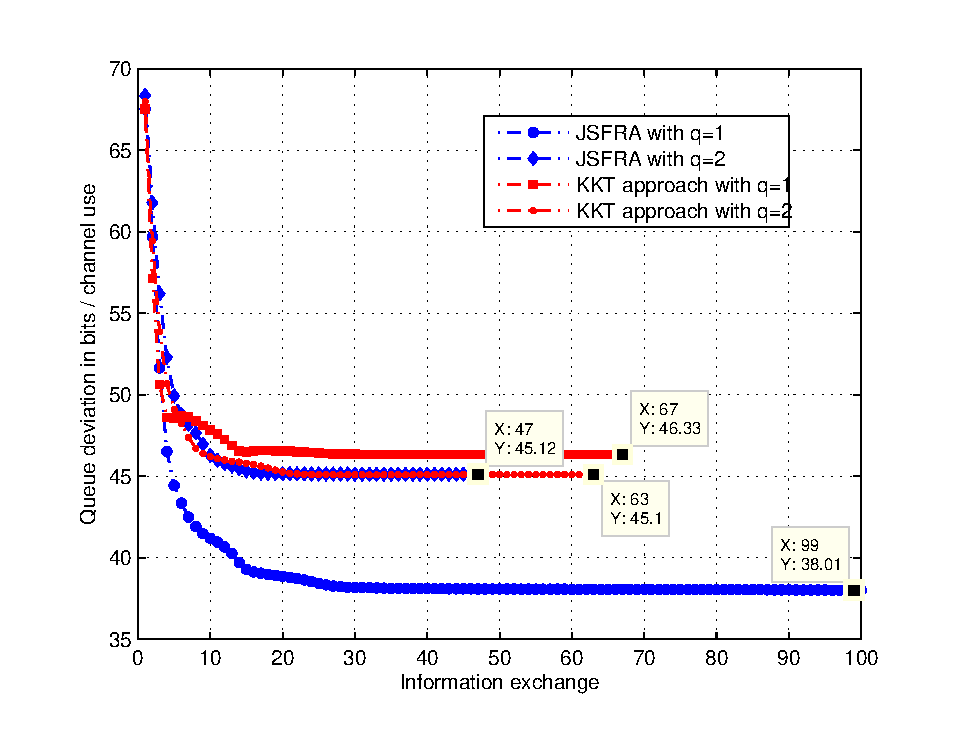
\includegraphics[width=\textwidth]{fig-7}
\caption{Queue deviation}
\end{subfigure}
\hfill
\begin{subfigure}{0.49\textwidth}
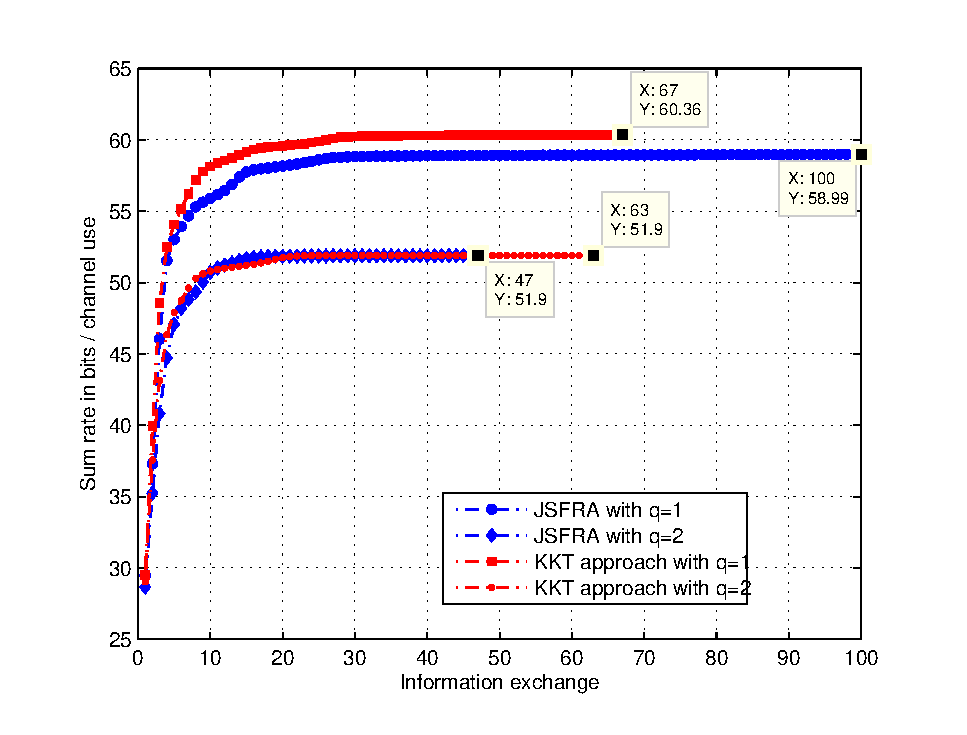
\includegraphics[width=\textwidth]{fig-8}
\caption{Sum rate performance}
\end{subfigure}
%\caption{Convergence plot for \me{\lbrace N,N_B,K,N_R \rbrace = \lbrace 6,3,12,1 \rbrace} model}
\caption{Convergence plot for \me{\lbrace N,N_B,K,N_R \rbrace = \lbrace 4,2,12,1 \rbrace} model}
\label{fig-d-3}
\end{figure*}
